\chapter{Human Driver Modelling}

In this chapter, the human driver model that Salvucci presents in \cite{salvucci_1} is implemented and the metrics used to verify the model are established. Initially, the model is implemented in \textit{Matlab} using the continuous driver model. To be able to verify it using the probabilistic model checking techniques presented in Chapter 2, the model undergoes an abstraction process, out of which a discrete-time Markov chain is obtained using several different approaches and assumptions. Metrics are then established to be able to evaluate whether the model meets the requirements and how well the human performs in a given situation. Finally, a simulator is presented in Section~\ref{sec:simulator} in order to allow visualisation of paths in the model.

\section{Continuous Driver Model using ACT-R}

In order to obtain a continuous driver model, we interpret Salvucci's integrated driver model as presented in \cite{salvucci_1}. The scenario considered is the one Salvucci envisioned: a multilane highway with moderate (or low) traffic \cite{salvucci_1}. The model uses the three modules presented in Figure~\ref{fig:high_level_salvucci}, that is, monitoring, decision making and control. All these modules rely on the constant update of the environment, as some are based on visual perception or low-level perception cues. While the human model is presented clearly in \cite{salvucci_1}, the dynamics of the car (which is part of the environment) are left to the reader, as it is outside the scope of the paper. In that sense, some assumptions had to be made about the environment.

The main initial assumption is that the driver is perfectly aware of its surroundings, and thus it is able to obtain the positions of other vehicles (within a certain distance) and the near and far points perfectly (this assumption is challenged later in the abstraction process). It is also assumed that the vehicle the driver is using is directly controlled by the updating of any pertinent variables within the control module of the architecture (i.e. there is no intermediate system or separation). The environment is assumed to change at the same rate as a cycle of the ACT-R model.

The overall view of the system is presented in Figure~\ref{fig:driver_model_overview}. The information flow is marked using the dotted arrows, while the sequential flow of the program is marked in the filled, lighter gray ones. Both the monitoring and the decision making make use of the perception which corresponds to querying the environment for the information (e.g. near and far point or another vehicle's position). The control both queries and sends updated information (e.g. vehicle position) to the environment. Modules are updated sequentially, following the order: control, monitoring, decision making and environment (e.g. position, velocity and acceleration of other vehicles).

\vspace{1em}
\begin{figure}[h]
    \centering
    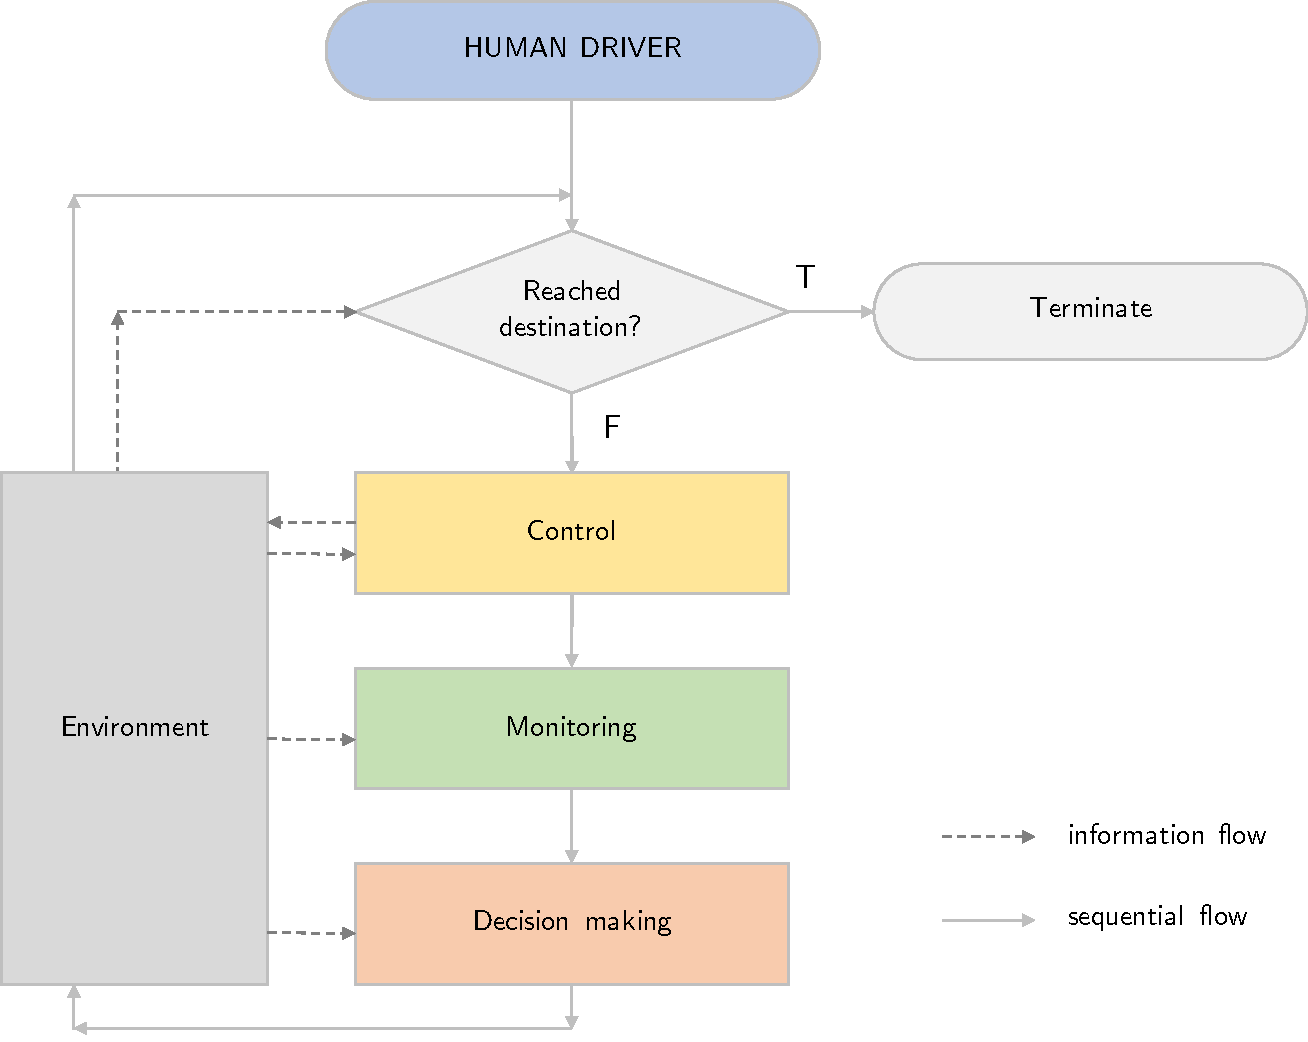
\includegraphics[width=0.85\textwidth]{matlab.pdf}
    \caption{Continuous Driver Model overview.}
    \label{fig:driver_model_overview}
\end{figure}

The monitoring module is implemented according to the flowchart presented in Figure~\ref{fig:monitor}, from the description given in \cite{salvucci_1}. The threshold for monitoring is set at $0.2$, as this is the value suggested in Salvucci in \cite{salvucci_1}. The output of this process corresponds to altering the global variable $a$ corresponding to the declarative memory cell composed of $k$ chunks. No specific value for $k$ is given by Salvucci in \cite{salvucci_1}, but it is taken to be 8 from \cite{lam}. The function \texttt{GET\_DISTANCE} is not described in depth due to the fact that it is trivial under the assumption stated in the previous paragraph.

The overall flowchart of the decision making module is shown in Figure~\ref{fig:dm}. The high level part is similar to the flowchart presented in Figure~\ref{fig:flowchart_dm}, with small differences related to the loading of variables and information from the different memories available. It is worth noticing that the control makes use of the function \texttt{LOOK\_VEHICLE} initially presented in the monitoring module to verify the presence of a vehicle in a relative position of a lane. The function \texttt{SET\_LANE\_FOLLOWING} is also omitted due to the trivial nature of this function under the assumptions made.

Finally, a flowchart for the control module is presented in Figure~\ref{fig:control}. This module is responsible for the calculation of $\Delta\varphi(t)$ and $\Delta\psi(t)$ and the update of the position. Given these two values, the position is updated following discrete laws of motion applied to rigid objects:

\begin{equation}
\begin{aligned}
	& \mathbf{v}(t) = \mathbf{v}(t-1) + \mathbf{a}(t)\Delta t\\
	& \mathbf{x}(t) = \mathbf{x}(t-1) + \mathbf{v}(t-1)\Delta t + \frac{1}{2}  \mathbf{a}(t)\Delta t^2 \\
	& t = t + \Delta t
\end{aligned}
\end{equation}

where $\mathbf{x}(t) = (x(t), y(t))$, $\mathbf{v}(t) = (v_x(t), v_y(t))$, and $\mathbf{a}(t) = (a_x(t), a_y(t))$, with:

\begin{equation}
\begin{aligned}
	a_x(t) & = \Delta\psi(t) \\
	a_y(t) & = \sin(\Delta\varphi(t))
\end{aligned}
\end{equation}

\begin{figure}
\centering
\begin{subfigure}{1\textwidth}
  \centering
  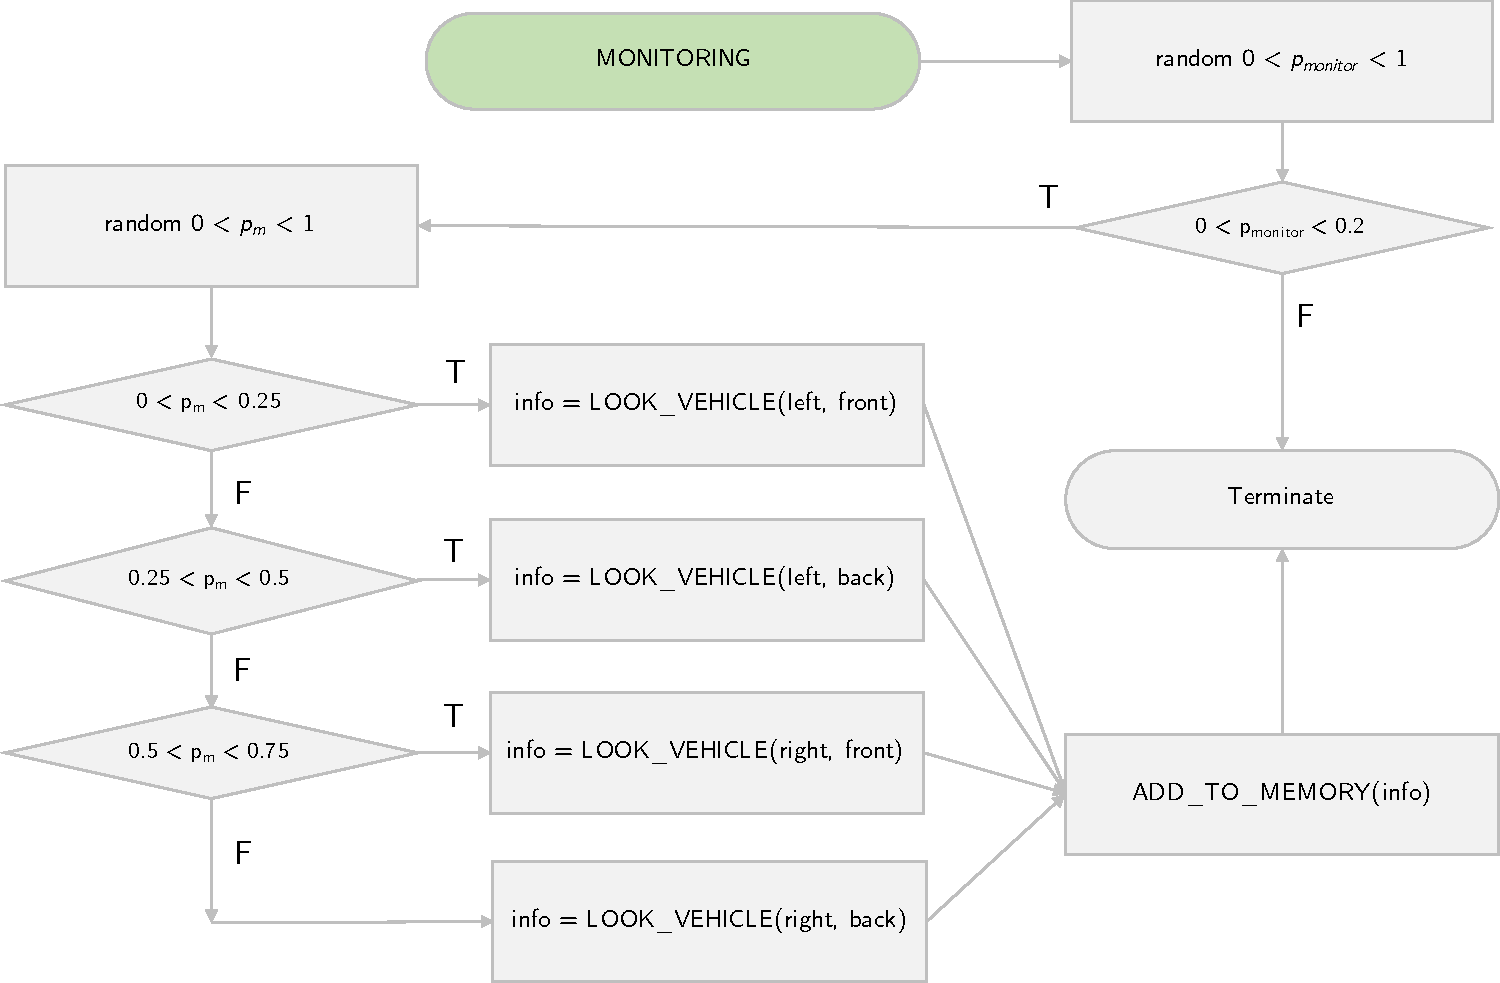
\includegraphics[width=1\textwidth]{monitor_1.pdf}
\end{subfigure}\\ \vspace{2em}
\begin{subfigure}{1\textwidth}
  \centering
  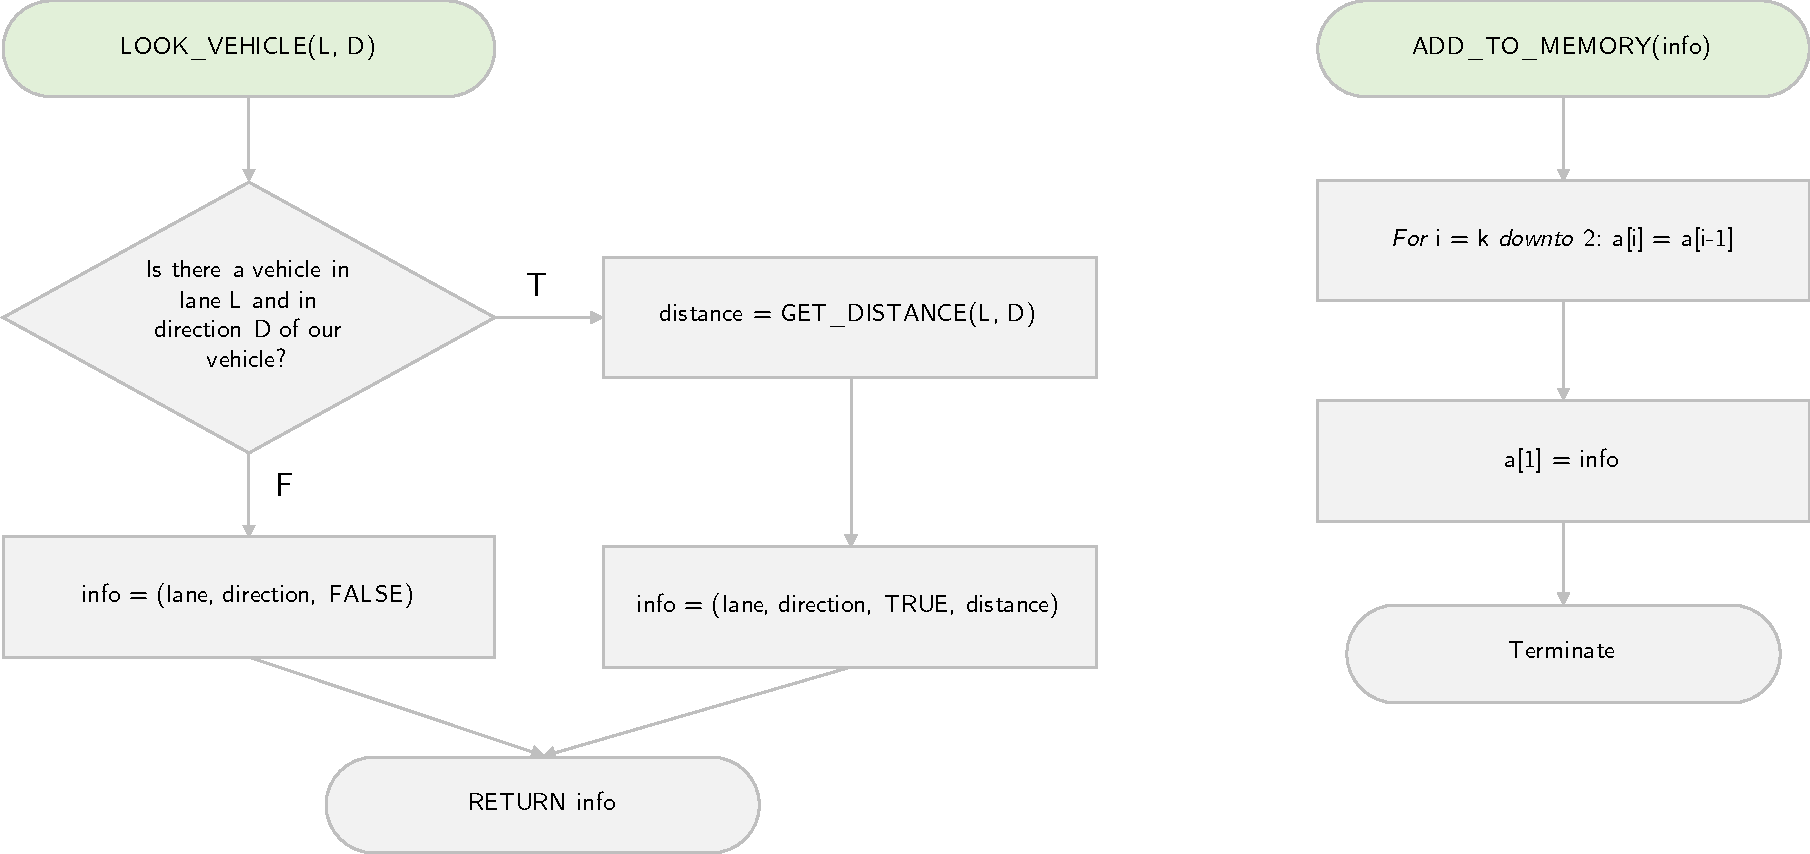
\includegraphics[width=1\linewidth]{monitor_2.pdf}
\end{subfigure} \vspace{2em}
\caption{Flowchart of the Monitoring module.}
\label{fig:monitor}
\end{figure}

\begin{figure}
\centering
\begin{subfigure}{1\textwidth}
  \centering
  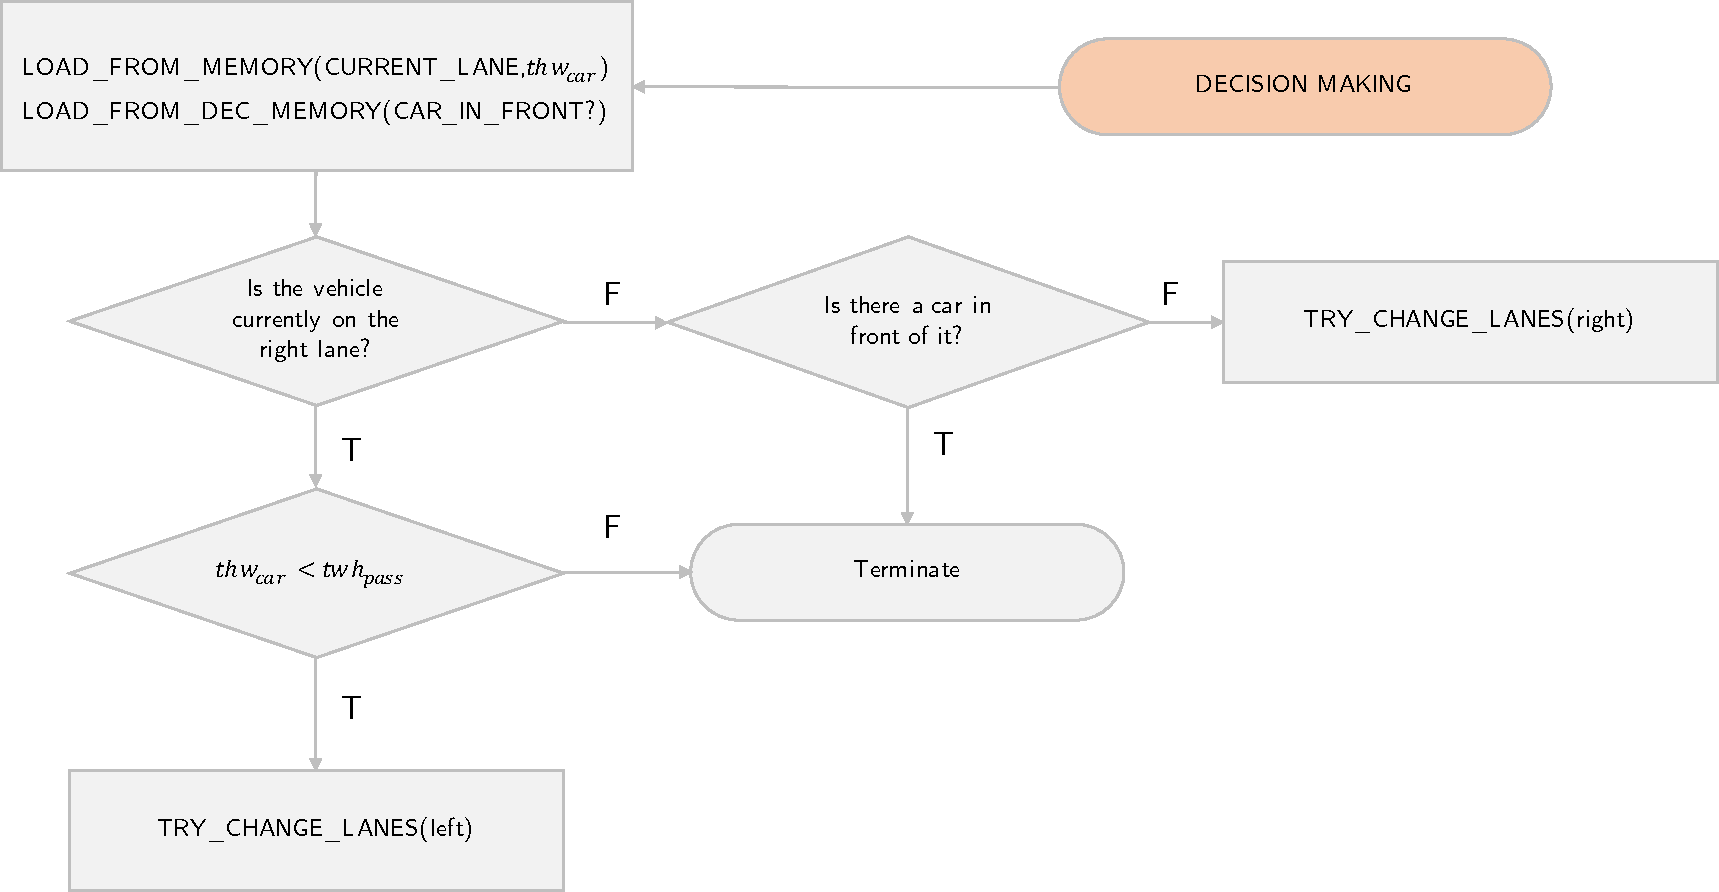
\includegraphics[width=1\textwidth]{dm_1.pdf}
\end{subfigure}\\ \vspace{2em}
\begin{subfigure}{1\textwidth}
  \centering
  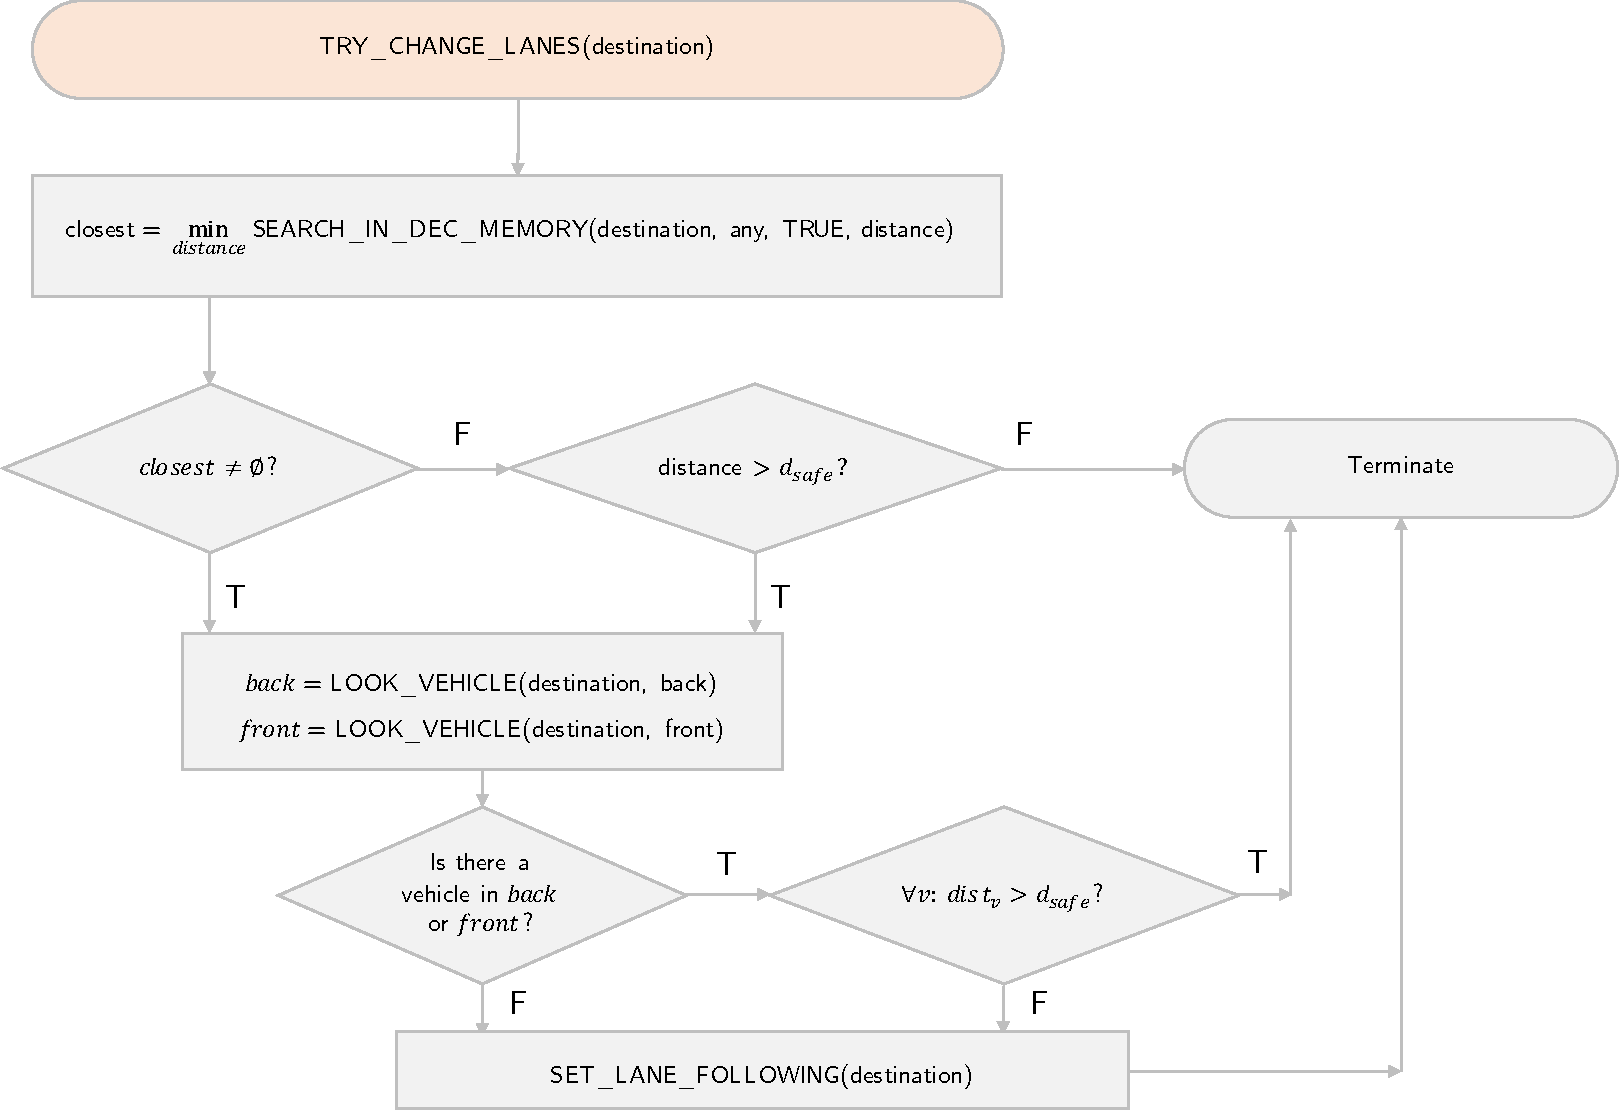
\includegraphics[width=1\linewidth]{dm_2.pdf}
\end{subfigure} \vspace{2em}
\caption{Flowchart of the Decision Making module.}
\label{fig:dm}
\end{figure}

\begin{figure}
\centering
\begin{subfigure}{1\textwidth}
  \centering
  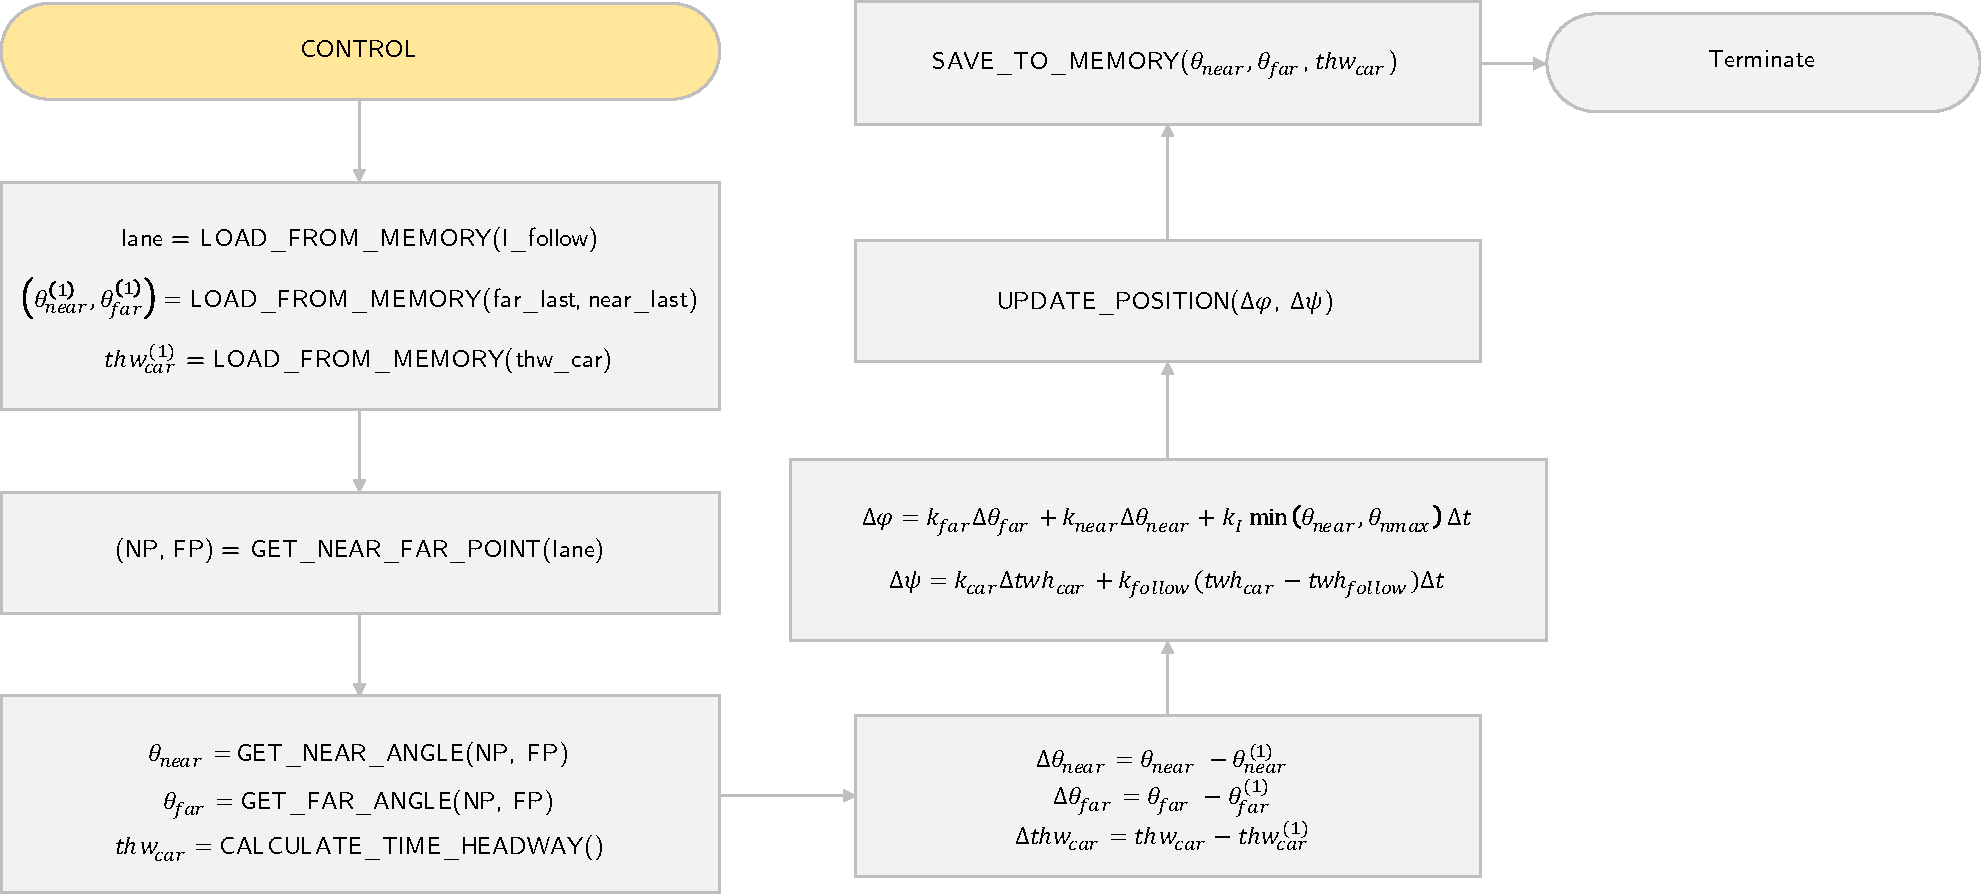
\includegraphics[width=1\textwidth]{control_1.pdf}
\end{subfigure}\\ \vspace{2em}
\begin{subfigure}{1\textwidth}
  \centering
  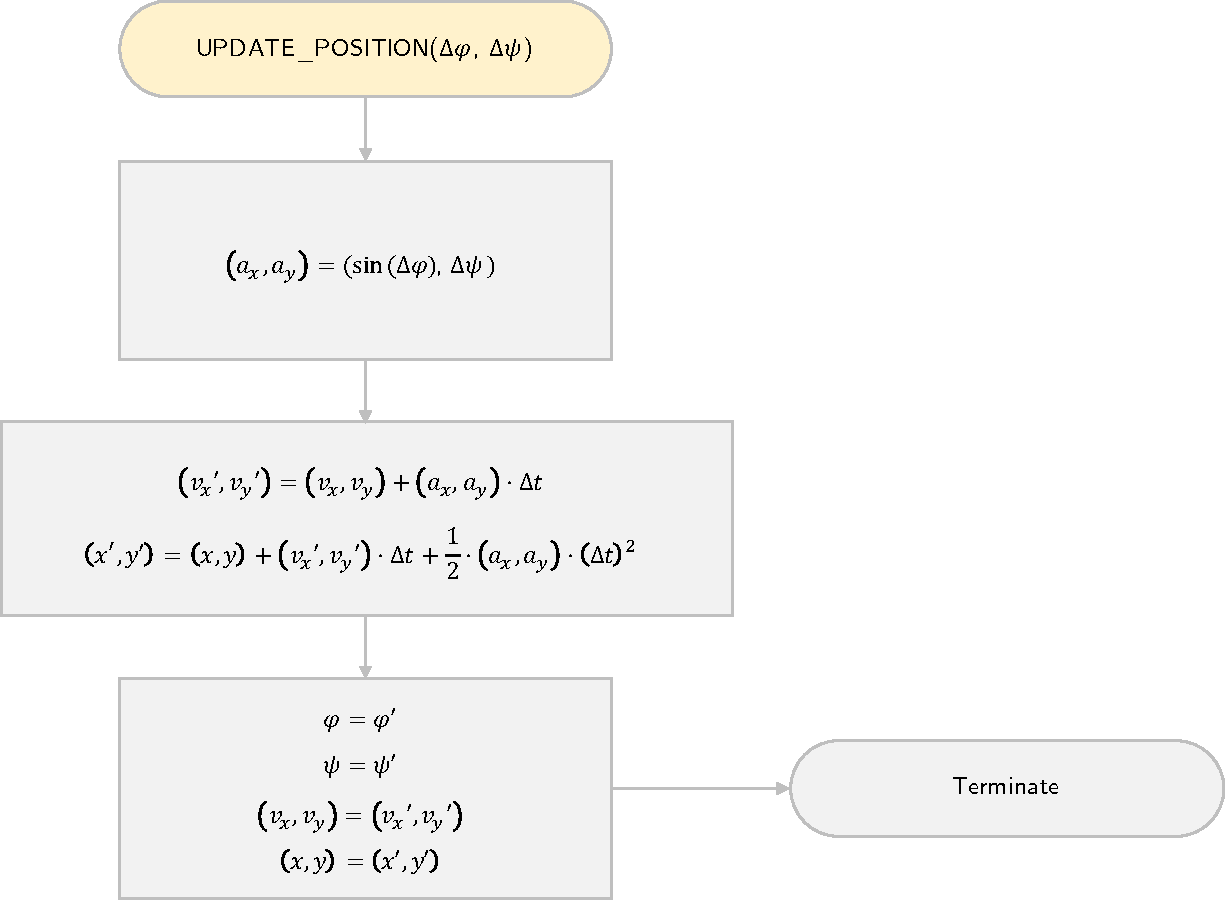
\includegraphics[width=0.7\linewidth]{control_2.pdf}
\end{subfigure} \vspace{2em}
\caption{Flowchart of the Control module.}
\label{fig:control}
\end{figure}

In this case, as Salvucci mentions in \cite{salvucci_1}, $\Delta t = 0.5s$. It is also assumed that the vehicle does not speed, and therefore, $v_x \in [15, 34]\text{ }m/s$ (between $50km/h$ and $120km/h$ - typical limits in highway speeds).

Using these assumptions, the continuous driver model is implemented in \textit{Matlab} as presented in Appendix~\ref{sec:appendix_cont}.

\section{Model Abstraction}

The process of abstraction consists in transforming the evolution of the continuous variables that constitute the model presented and discretising it in order to obtain a finite discrete model. In this case, the goal is to go from the continuous model of driver behaviour presented in the previous section to a discrete-time Markov chain (DTMC) which represents the same process. This transformation is less than trivial due to the fact that, in model checking of finite state abstractions, as the number of state variables in the system increases, the size of the system state space grows exponentially \cite{state_explosion}. This problem is known as state explosion, and there has been some research into efficient ways of dealing with it \cite{abstraction_1, abstraction_2}. 

In the following sections, the abstraction process for the different modules of ACT-R is presented in detail, as well as the thought process behind the choices made.

\subsection{Non-Probabilistic Control Module}

The control module, as presented in the previous section and following Salvucci's approach in \cite{salvucci_1}, is fully deterministic, in the sense that there is no probabilistic reasoning involved. It makes use of perception (for the near and far points) and two simple control laws which influence the position, velocity and acceleration of the vehicle in the environment.

The straightforward approach to this problem would be to represent it as a simple grid $N\times M$, in which a tuple $(x,y)$ with $x\in \{0,...,N\}$ and $y\in \{0,...,M\}$ would describe the position of the vehicle and all other variables (i.e. $v_x$, $v_y$, $a_x$, $a_y$ and $t$) would be integer versions of its continuous model representation. In this approach, the control laws could be applied directly over the grid and the results would be the movement of the vehicle in it. However, there is an intrinsic problem with this approach. The error associated with the use of the grid as a way to discretise space would, logically, be reduced with an increase of the $N$ and $M$ for a representation of the same segment (i.e. increase in resolution). For example, the error associated with a road segment of $500 \times 7m^2$ represented by $N = 500$ and $M = 7$ (each grid square corresponds to $1m^2$) would be significantly greater than if $N = 5000$ and $M = 70$ (each grid square corresponds to about $10^{-2}\text{ }m^2$). The conclusion would be that one should increase $N$ and $M$ in order to obtain an appropriate resolution, but this incurs in the problem of state explosion presented in the beginning of the section: as the variable ranges increase, the number of states in the system grows exponentially. Thus, while the situation of $N = 5000$ and $M = 70$ is appealing in terms of error, it would be intractable to actually build and perform model checking on it (e.g. for $v_x, v_y \in \{15,...,34\}^2$ and $a_x, a_y \in \{-3,...,3\}^2$, the state space of the control module alone would have approximately $6.89\times 10^{9}$ states, making it impossible to add decision making and monitoring). 

The straightforward strategy is not, by any standards, efficient in terms of state space and does not use any of the information of the problem to simplify it. In particular, one should notice in this case that the movement in the $y$ direction is used simply for the purpose of lane changing, a process which is purely deterministic (as described in \cite{salvucci_1}). Therefore, a more interesting approach to the abstraction of the control module could take this into account and \textbf{pre-simulate the lane changing operations}.

In this approach, the vehicle's position is represented by two variables $x \in \{0,...,N\}$ for a given $N$ and $lane \in \{right, left\}$ (can be extended to more than two lanes), and the acceleration and velocity of the vehicle are simply $a = a_x$ and $v = v_x$. Time is still represented in the same way, with $t \in \{0,...,max\_time\}$ If a lane change is decided by the decision making module, then, within one transition, the $lane$ variable switches its value and the variables $x, v, a$ and $t$ are updated to reflect this. These values are obtained from a look-up table and depend on the distance to the obstacle/vehicle in front of it ($d$) and the velocities of both the vehicle in question ($v$) and the obstacle/vehicle ($v_1$). Additionally, a variable $crashed$ is used to represent whether a vehicle has crashed in the process or not. The linear acceleration is implemented similarly using pre-simulation to determine the value of acceleration and the motion law is updated in the model itself.

The continuous model of driver behaviour obtained in the previous section in \textit{Matlab} is used as basis for the simulation of lane changes and linear acceleration. From this model, the look-up tables are obtained which, given an origin lane ($o_{lane}$), a distance to the lead vehicle and the velocities of both the vehicle in question and the lead vehicle determines whether a crash happened or not, what is the $\Delta x$ and $\Delta T$ incurred (how did the position in $x$ changed and how long did it take), and the final velocity of the vehicle in question. The code presented in Appendix~\ref{sec:control_abs} corresponds to a similar version of the control (but probabilistic, as presented later in this section). An example of the simulation of the scenario $o_{lane} = 1$, $d = 20m$, $v = 15m/s$ and $v_1 = 20m/s$ is shown in Figure~\ref{fig:lane_change_ex}.

\begin{figure}[h]
    \centering
    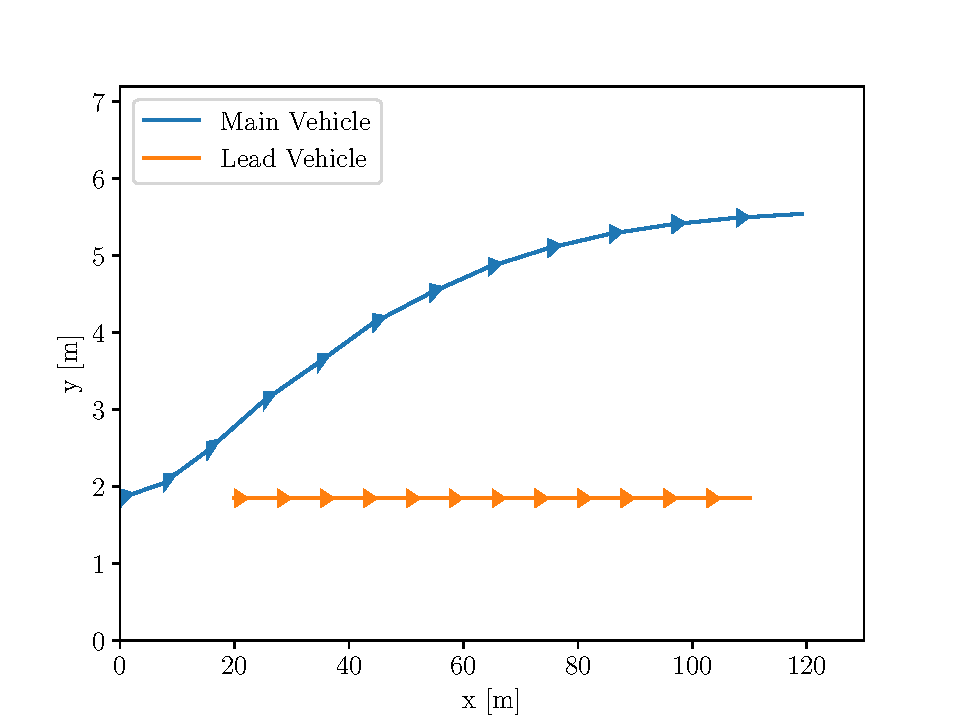
\includegraphics[width=0.9\textwidth]{lane_change_ex.pdf}
    \caption{Example of the simulation of the lane change for $o_{lane} = 1$ (left lane), $d = 20m$, $v = 15m/s$ and $v_1 = 15m/s$. In this case, after the change is complete the variable assignments are $crashed = 0$ (no collision happened), $\Delta x = 119m$, $\Delta T = 6s$ and $v = 23m/s$.}
    \label{fig:lane_change_ex}
\end{figure}

This focuses the computational effort on the pre-calculations, simplifying the final model significantly in terms of the state space, while removing the error made by discretising in the $y$ direction of the grid (the error in the $x$ direction is still present though). With regards to the size of the lane changing table, for the considered scenario of $2$ lanes, $v, v_1 \in \{15,...,34\}^2$ and for any discrete $d \in \{0,...N\}$, the size of the table would be $2\times 20^2 \times N = 800 \times N$. Given that the only value of the table that is effectively altered with a change in $d$ is the value of $crashed$ (as the $\Delta x$, $\Delta t$ and final $v$ depend solely on the initial velocities of both vehicles), the table can consider:

\begin{equation}
d_{\max} < N\text{, s.t. }\forall v, v_1 \in \{15,...,34\}^2, d' \geq d_{\max}: crashed_{d'} = false
\end{equation}

that is, a great enough value of $d$ such that, regardless of the speed of the two vehicles, no crash will occur between them. For the given ranges of $v$ and $v_1$, $d_{\max}$ is determined to be $43$, and thus the obtained look-up table contains $34,400$ rows.

The linear acceleration table depends on the $thw_{car}$ which varies only with the distance to the front vehicle and the current velocity of the vehicle. Considering the distance in this case to be up to $80 m$ (otherwise maximum acceleration will be applied), the look-up table generated has $1,600$ rows.

\subsection{Decision Making and Monitoring Module}

Due to the fact that, in the model presented by Salvucci in \cite{salvucci_1}, the monitoring module influences the declarative memory which is then used exclusively for decision making purposes (and not for control), logically these two can be incorporated into one for abstraction purposes. Again, taking the straightforward approach of trying to include the declarative memory and the process associated with monitoring and decision making into the model directly would make it intractable. 

In its simplest form, the decision making process localises the car and decides whether or not to change lanes based on the time headway, $thw_{car}$, to the car in front of it (if there is one). This value essentially corresponds to the time the main vehicle has before it crashes into the vehicle in front of it, assuming that vehicle came to a full stop ($v = a = 0$) \cite{thw}. The lower this time headway, the more likely a driver is to perform the manoeuvre. While Salvucci presents a fully deterministic driver in \cite{salvucci_1} based on the average driver, in this dissertation it was decided to try and analyse drivers according to different profiles in order to simulate how different parts of the population of drivers might make decisions. The decision making in such a case follows from a stochastic reasoning which can be simulated and incorporated in the model using look-up tables. In this case, it was decided to model the probability of a driver performing a lane change based on the time headway could be modelled using an exponentially decreasing function, such as:

\begin{equation}
	\text{P[}lC = true\text{]}_{thw} = P_{lC}(d,v) = e^{-\alpha\cdot thw} = e^{-\alpha\cdot d/v}
\end{equation}

where $\alpha$ is a parameter unique to each population of drivers. It should be noted that this function, while logical, is an assumption of the abstraction, since the model presented by Salvucci in \cite{salvucci_1} does not make any reference to this parameterisation. It is also worth referring that, while there was no real-world data involved in this project, this function can be learned from real data without changing the fundamental paradigm of the abstraction.

For the purposes of analysis, three classes of drivers are considered: \textbf{Aggressive}, \textbf{Average} and \textbf{Cautious} drivers (with different values for the parameter $\alpha$). In Figure~\ref{fig:dm_curve}, the functions are presented for the three profiles of drivers assumed in this project.

\begin{figure}[h]
    \centering
    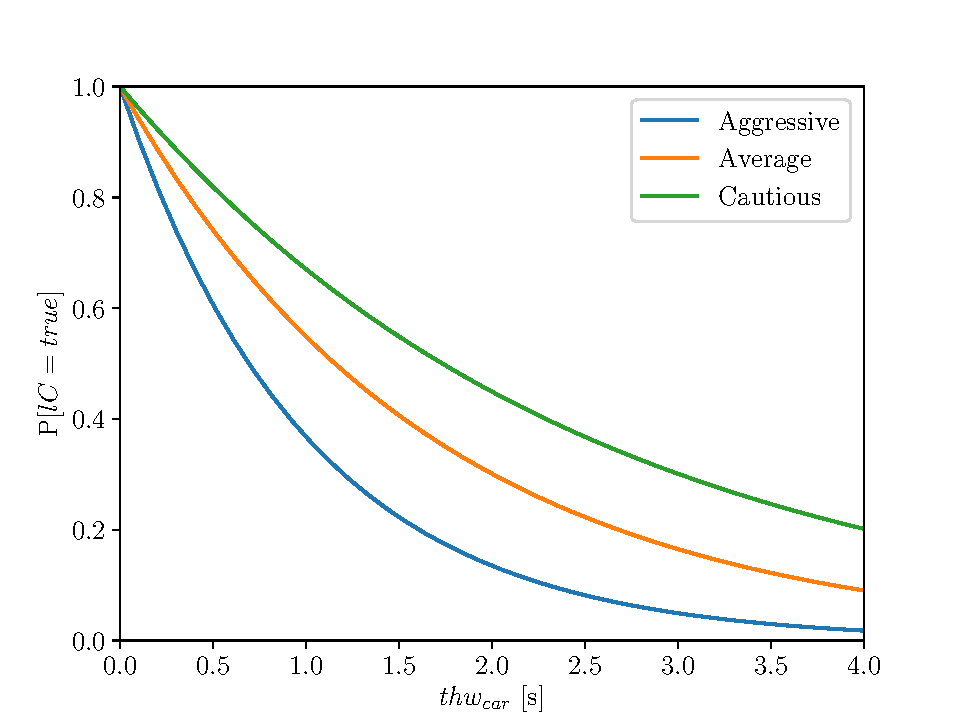
\includegraphics[width=0.9\textwidth]{dm_curve.pdf}
    \caption{$\text{P[}lC = true\text{]}$ as a function of $thw_{car}$ for Aggressive ($\alpha = 1$), Average ($\alpha = 0.6$) and Cautious ($\alpha = 0.4$) drivers.}
    \label{fig:dm_curve}
\end{figure}

However, this corresponds to a version of decision making which is not influenced by the monitoring module at all, and it relies on the correct calculation of the value of $thw_{car}$. This assumption is unrealistic, and in order to simulate these issues, it was decided that stochastic noise could be added to the measurement of the distance (as this is what human drivers have to instinctively measure through perception). It was chosen that this noise, $n$, would be normally distributed as:

\begin{equation}
	n \sim \mathcal{N}(0, \sigma)
\end{equation}

such that:

\begin{equation}
	thw'_{car} = thw_{car} + n(thw_{car})
\end{equation}

Alternatively, this can be represented directly as (using integration steps of 1):

\begin{equation}
\begin{aligned}
	P'_{lC}(d,v) & = \sum_{i = -\infty}^{+\infty} [N(d + i + 0.5) - N(d + i - 0.5)] \cdot P_{lC}(d + i,v) \\
	& = \sum_{i = -\max_d}^{+\max_d} [N(d + i + 0.5) - N(d + i - 0.5)] \cdot P_{lC}(d + i,v)
\end{aligned}
\end{equation}

where $\max_d$ is the maximum length considered and $N(d)$ corresponds to the cumulative probability function (CDF) defined as:

\begin{equation}
	N(d) = \int_{-\infty}^d n(t) dt
\end{equation}

From this, a look-up table can be generated which, for different driver types, yields the probability of lane changing for a certain distance to the lead car and velocity. For the 3 driver profiles mentioned, considering $d \in \{1,...,80\}$ ($\max_d = 80$) and $v \in \{15,...,34\}$, the table generated has $4,800$ rows.

The same logic can be applied for a driver in the left lane overtaking a vehicle behind it in the left lane, except in this case the opposite effect will be seen in the decision making. In such a case, the probability of changing lane can be modelled as a normalised logarithmic function over the distance of the vehicles (it doesn't make sense to define time headway in this context):

\begin{equation}
	\text{P[}lC = true\text{]}_{d} = P_{lC}(d) = \frac{1}{\log(\beta*\max_d + 1)}\cdot \log(\beta*d + 1)
\end{equation}

where $\max_d$ is the maximum length considered and $\beta$ is a parameter unique to each population of drivers. In Figure~\ref{fig:dm_curve_2}, the functions are presented for the three profiles of drivers previously mentioned.

\begin{figure}[h]
    \centering
    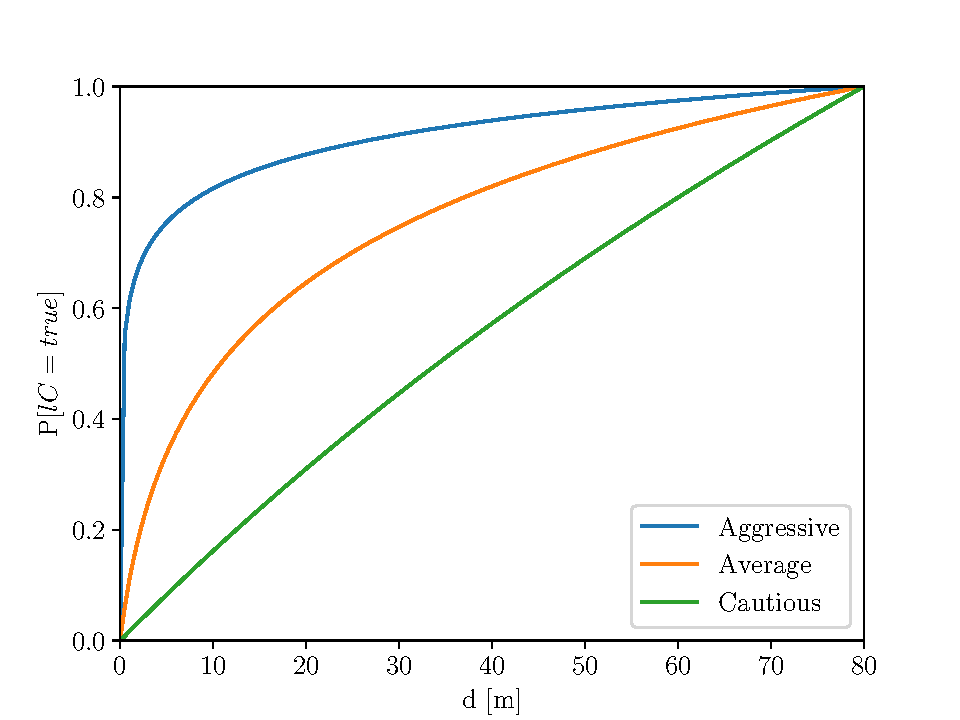
\includegraphics[width=0.9\textwidth]{dm_curve_2.pdf}
    \caption{$\text{P[}lC = true\text{]}$ as a function of $d$ for Aggressive ($\beta = 1000$), Average ($\beta = 0.5$) and Cautious ($\beta = 0.01$) drivers.}
    \label{fig:dm_curve_2}
\end{figure}

For the 3 driver profiles mentioned, considering $d \in \{1,...,80\}$ ($\max_d = 80$), this look-up table obtained has $240$ rows. The unified decision making table has, therefore, $5,040$ rows.

The code presented in Appendix~\ref{sec:dm_abs} corresponds to the methods to obtain the look-up tables mentioned regarding the decision making and monitoring module.

\subsection{Probabilistic Control Module}

In light of the uncertainty introduced in the decision making and monitoring module regarding the visual perception of distance, it becomes only natural that this would be extended to the control module as well. In order to cope with this, a probabilistic version of the control module was designed, where the noise $n$ presented in the previous subsection is taken into consideration. 

In order to obtain the equivalent look-up table for the probabilisitic control module, the noise can be simulated using repeated trials, and an average can be obtained for the crashing probability, the estimated final difference in position, the estimated difference in time and estimated final velocity of the vehicle. In the case of this dissertation, the tables generated (for linear and lane changing control) were the result of 100 trials.

The code presented in Appendix~\ref{sec:control_abs} corresponds to the simulation of this probabilistic version of the control.

\subsection{Unified Two-Module Model}

Using the three tables generated (two for the probabilisitic control - linear and steering control - and one for the decision making), the final DTMC model unifies both using a sequential variable $actr\_state \in \{1,2\}$, where $actr\_state = 1$ corresponds to the control and $actr\_state = 2$ corresponds to decision making. In the unified model, only two vehicles are present: one is the one controlled by the driver and another one starts at a distance $x = x_{1,0}$ from the main vehicle (which starts at $x=0$) and moves with a constant speed of $v_1$. Its movement is, therefore, completely determined by the formula:

\begin{equation}
	x_1(t) = x_{1,0} + v_1\cdot t
\end{equation}

The distance between the two vehicles can be written as:

\begin{equation}
	d(t) = \lvert x(t) - x_1(t) \rvert
\end{equation}

And the boolean function $posDist$ can be defined as:

\begin{equation}
posDist(t) = 
     \begin{cases}
       \text{true,} &\quad\text{if }x(t) \geq x_1(t)\\
       \text{false,} &\quad\text{otherwise.} \\
     \end{cases}
\end{equation}

Due to the size of the tables generated, the models should be generated automatically for a given tuple of initial conditions $(d_{type}, v, v_1, x_{1,0})$ (where $d_{type}$ is the driver class according to the ones defined in the decision making and monitoring subsection - 1 is aggressive, 2 is average and 3 is cautious), following a set of assumptions:

\begin{enumerate}
	\item A transition between two states $s$ and $s'$ is possible if, and only if, the variable $actr\_state$ takes different values in $s$ and $s'$.
	\item If the vehicle has crashed, the model enters a deadlock.
	\item If the vehicle is on the left lane and behind the other vehicle, it will not attempt a lane change.
	\item If the vehicle is on the right lane and in front of the other vehicle, it will not attempt a lane change.
\end{enumerate}

From these, it is possible to build a model generator, as presented in Appendix~\ref{sec:two_module_gen}. 

By running the model generator using the conditions $(d_{type}, v, v_1, x_{1,0}) = (1,30,22,51)$, that is, an aggressive driver, starting at $30m/s$ with another vehicle going at $22m/s$ and starting at $51m$, the resulting model is the one presented in Listing~\ref{lst:model_example} (in PRISM Language).

{\vspace{1em}
\begin{lstlisting}[caption={Example of the model generated for the tuple $(d_{type}, v, v_1, x_{1,0}) = (1,30,22,51)$ (shortned)},captionpos=b,label={lst:model_example}]
//Model automatically built using model_generator.py for v1 = 22 and driver_type = 1 (to alter these values, run the script again).
//Generated on 31-07-2018 at 18:47.

dtmc

const int length = 500; // road length
const int driver_type = 1; // 1 = aggressive, 2 = average, 3 = cautious drivers - do not alter this manually!
const int max_time = 35; // maximum time of experiment

// Other vehicle
const int v1 = 22; // do not alter this manually!
const int x1_0 = 51;

// Environment variables
global t : [0..max_time] init 0; // time 
global crashed : bool init false; 

// Vehicle controlled
global actrState : [1..2] init 1; // active module: 1 = control (both cars), 2 = decision making + monitoring
global lC : bool init false; // lane changing occuring? 
global x : [0..length] init 0;
global v : [15..34] init 30;
global a : [-2..3] init 0;
global lane : [1..2] init 1;

formula x1 = x1_0 + v1*t;
formula dist = x1>x?(x1 - x):(x - x1);
formula positiveDist = (x < length)?x > x1:true;

module Decision_Making_Monitoring

 	// If a crash occurs, then nothing else can happen
	//[] actrState = 2 & crashed -> 1:(crashed' = true);

 	// If we are in lane 2, but behind the other vehicle, don't try to pass
	[] actrState = 2 & !crashed & lane = 2 & positiveDist = false -> 1:(actrState' = 1);

	// If we are in lane 1, and no vehicle is in front, don't change lanes
	[] actrState = 2 & !crashed & lane = 1 & positiveDist = true -> 1:(actrState' = 1);

	[] actrState = 2 & !crashed & lane = 1 & positiveDist = false & dist = 1 & v = 15 -> 0.8:(actrState' = 1) & (lC' = true) + 0.2:(actrState' = 1) & (lC' = false);

	...

	[] actrState = 2 & !crashed & lane = 2 & positiveDist = true & dist >= 80 -> 1:(actrState' = 1) & (lC' = true) + 0:(actrState' = 1) & (lC' = false);
endmodule

module Control

 	// If we are in lane 1, and no lane change was decided, continue forward (which might result in crash)
 	// The vehicle is behind the other driver (positiveDist = false, x < x1)
	[] actrState = 1 & !crashed & !lC & lane = 1 & x <= length - v & t < max_time & positiveDist = false & (x1 + v1 - x - v) >= 6 & v + a < 34 & v + a > 15 & dist = 1 & v = 15  -> 1:(x' = x + v) & (t' = t + 1) & (v' = v + a) & (a' = -2) & (actrState' = 2);

	...

	[] actrState = 1 & !crashed & lC & lane = 2 & dist >= 43 & v = 34 & x > length - 136 & t > max_time - 6 -> 1:(crashed' = false) & (x' = length) & (v' = 34) & (t' = max_time) & (a' = 0) & (lane' = 1) & (actrState' = 2) & (lC' = false);

endmodule
\end{lstlisting}
}

By loading and building the model in either PRISM or Storm, it is observable that it has 257 states and 295 transitions, corroborating the assumption that the abstraction methods used returned efficient outcomes. Due to the fact that there are $3\times 20 \times 20 \times \text{length}$ (where length is the size of the road segment considered in meters) different possibilities in terms of initial conditions, it would be intractable, in the timeline of the dissertation, to obtain the number of states for all the combinations. Table~\ref{tab:sta_tra_example} presents the number of states and transitions for some arbitrarily generated conditions.

\bgroup
\def\arraystretch{1.3}
\begin{table}[h]
\centering
\begin{tabular}{|c|c|c|c||c|c|}
\hline
\textbf{$d_{type}$} & \textbf{$v$} & \textbf{$v_1$} & \textbf{$x_{1,0}$} & \textbf{\# States} & \textbf{\# Transitions} \\ \hline \hline
3 & 21 & 30 & 20 & 305 & 333 \\ \hline
1 & 27 & 22 & 66 & 396 & 471 \\ \hline
1 & 28 & 17 & 43 & 167 & 183 \\ \hline
2 & 33 & 15 & 35 & 6 & 7 \\ \hline
3 & 28 & 21 & 38 & 199 & 222 \\ \hline
1 & 19 & 16 & 81 & 391 & 443 \\ \hline
2 & 25 & 23 & 28 & 390 & 481 \\ \hline
\end{tabular}
\caption{Results of the number of states and transitions for arbitrary initial conditions.}
\label{tab:sta_tra_example}
\end{table}
\egroup

\section{Model Evaluation Metrics}

Lorem ipsum dolor sit amet, consectetur adipiscing elit. Pellentesque accumsan magna eu metus congue, vitae tristique enim commodo. Aliquam consectetur porttitor nisl, eget pulvinar quam venenatis eget. Aliquam erat volutpat. Nullam at ipsum at felis tincidunt consequat non sed mi. Morbi placerat iaculis dapibus. Aliquam non risus ac urna interdum pretium. Donec maximus, massa vitae suscipit congue, ligula purus sagittis magna, vitae interdum enim dui sed felis. Curabitur mollis eleifend diam a varius. Vivamus eu porttitor lorem. Mauris sagittis ultrices ligula, a euismod mi efficitur a. Aenean molestie sapien a nibh suscipit, nec venenatis urna varius. Sed eu ex id lacus tincidunt ultricies. Aenean quam massa, dignissim ac suscipit posuere, varius sit amet turpis. Nunc semper turpis ullamcorper elit venenatis, in molestie nulla fermentum.

\subsection{Completeness Property}

Lorem ipsum dolor sit amet, consectetur adipiscing elit. Pellentesque accumsan magna eu metus congue, vitae tristique enim commodo. Aliquam consectetur porttitor nisl, eget pulvinar quam venenatis eget. Aliquam erat volutpat. Nullam at ipsum at felis tincidunt consequat non sed mi. Morbi placerat iaculis dapibus. Aliquam non risus ac urna interdum pretium. Donec maximus, massa vitae suscipit congue, ligula purus sagittis magna, vitae interdum enim dui sed felis. Curabitur mollis eleifend diam a varius. Vivamus eu porttitor lorem. Mauris sagittis ultrices ligula, a euismod mi efficitur a. Aenean molestie sapien a nibh suscipit, nec venenatis urna varius. Sed eu ex id lacus tincidunt ultricies. Aenean quam massa, dignissim ac suscipit posuere, varius sit amet turpis. Nunc semper turpis ullamcorper elit venenatis, in molestie nulla fermentum.

\subsection{Safety Property}

Lorem ipsum dolor sit amet, consectetur adipiscing elit. Pellentesque accumsan magna eu metus congue, vitae tristique enim commodo. Aliquam consectetur porttitor nisl, eget pulvinar quam venenatis eget. Aliquam erat volutpat. Nullam at ipsum at felis tincidunt consequat non sed mi. Morbi placerat iaculis dapibus. Aliquam non risus ac urna interdum pretium. Donec maximus, massa vitae suscipit congue, ligula purus sagittis magna, vitae interdum enim dui sed felis. Curabitur mollis eleifend diam a varius. Vivamus eu porttitor lorem. Mauris sagittis ultrices ligula, a euismod mi efficitur a. Aenean molestie sapien a nibh suscipit, nec venenatis urna varius. Sed eu ex id lacus tincidunt ultricies. Aenean quam massa, dignissim ac suscipit posuere, varius sit amet turpis. Nunc semper turpis ullamcorper elit venenatis, in molestie nulla fermentum.

\subsection{Liveness Properties}

Lorem ipsum dolor sit amet, consectetur adipiscing elit. Pellentesque accumsan magna eu metus congue, vitae tristique enim commodo. Aliquam consectetur porttitor nisl, eget pulvinar quam venenatis eget. Aliquam erat volutpat. Nullam at ipsum at felis tincidunt consequat non sed mi. Morbi placerat iaculis dapibus. Aliquam non risus ac urna interdum pretium. Donec maximus, massa vitae suscipit congue, ligula purus sagittis magna, vitae interdum enim dui sed felis. Curabitur mollis eleifend diam a varius. Vivamus eu porttitor lorem. Mauris sagittis ultrices ligula, a euismod mi efficitur a. Aenean molestie sapien a nibh suscipit, nec venenatis urna varius. Sed eu ex id lacus tincidunt ultricies. Aenean quam massa, dignissim ac suscipit posuere, varius sit amet turpis. Nunc semper turpis ullamcorper elit venenatis, in molestie nulla fermentum.

\section{Simulation of Paths in the Model}
\label{sec:simulator}

Lorem ipsum dolor sit amet, consectetur adipiscing elit. Pellentesque accumsan magna eu metus congue, vitae tristique enim commodo. Aliquam consectetur porttitor nisl, eget pulvinar quam venenatis eget. Aliquam erat volutpat. Nullam at ipsum at felis tincidunt consequat non sed mi. Morbi placerat iaculis dapibus. Aliquam non risus ac urna interdum pretium. Donec maximus, massa vitae suscipit congue, ligula purus sagittis magna, vitae interdum enim dui sed felis. Curabitur mollis eleifend diam a varius. Vivamus eu porttitor lorem. Mauris sagittis ultrices ligula, a euismod mi efficitur a. Aenean molestie sapien a nibh suscipit, nec venenatis urna varius. Sed eu ex id lacus tincidunt ultricies. Aenean quam massa, dignissim ac suscipit posuere, varius sit amet turpis. Nunc semper turpis ullamcorper elit venenatis, in molestie nulla fermentum.
